% !TeX spellcheck = en_GB
% !TeX encoding = UTF-8
% !TeX program = xelatex
% TODO Change language to en_GB (recommended) or en_US for English documents
\documentclass[11pt,a4paper,oneside]{report}             % Single-side
%\documentclass[11pt,a4paper,twoside,openright]{report}  % Duplex

% thanks to http://tex.stackexchange.com/a/47579/71109
\usepackage{ifxetex}
\usepackage{ifluatex}
\newif\ifxetexorluatex % a new conditional starts as false
\ifnum 0\ifxetex 1\fi\ifluatex 1\fi>0
   \xetexorluatextrue
\fi

\ifxetexorluatex
  \usepackage{fontspec}
\else
  \usepackage[T1]{fontenc}
  \usepackage[utf8]{inputenc}
  \usepackage[lighttt]{lmodern}
\fi

\usepackage[english,magyar]{babel} % Alapértelmezés szerint utoljára definiált nyelv lesz aktív, de később külön beállítjuk az aktív nyelvet.

%\usepackage{cmap}
\usepackage{amsfonts,amsmath,amssymb} % Mathematical symbols.
%\usepackage[ruled,boxed,resetcount,linesnumbered]{algorithm2e} % For pseudocodes. % beware: this is not compatible with LuaLaTeX, see http://tex.stackexchange.com/questions/34814/lualatex-and-algorithm2e
\usepackage{booktabs} % For publication quality tables for LaTeX
\usepackage{graphicx}

%\usepackage{fancyhdr}
%\usepackage{lastpage}

\usepackage{anysize}
%\usepackage{sectsty}
\usepackage{setspace} % For setting line spacing

\usepackage[unicode]{hyperref} % For hyperlinks in the generated document.
\usepackage{xcolor}
\usepackage{listings} % For source code snippets.

\usepackage[amsmath,thmmarks]{ntheorem} % Theorem-like environments.

\usepackage[hang]{caption}

\singlespacing

\newcommand{\selecthungarian}{
	\selectlanguage{magyar}
	\setlength{\parindent}{2em}
	\setlength{\parskip}{0em}
	\frenchspacing
}

\newcommand{\selectenglish}{
	\selectlanguage{english}
	\setlength{\parindent}{0em}
	\setlength{\parskip}{0.5em}
	\nonfrenchspacing
	\renewcommand{\figureautorefname}{Figure}
	\renewcommand{\tableautorefname}{Table}
	\renewcommand{\partautorefname}{Part}
	\renewcommand{\chapterautorefname}{Chapter}
	\renewcommand{\sectionautorefname}{Section}
	\renewcommand{\subsectionautorefname}{Section}
	\renewcommand{\subsubsectionautorefname}{Section}
}

\usepackage[numbers]{natbib}
\usepackage{xspace}

\usepackage{tikz}
\usetikzlibrary{shapes,arrows,decorations.markings}

\usetikzlibrary{positioning}
\tikzstyle{block} = [rectangle, draw,
    text width=7em, text centered,minimum height=3em,minimum width=8em]
    \tikzstyle{label} = [
    text width=5em, text centered]
\tikzstyle{block_rounded} = [rectangle, draw, 
    text width=5em, text centered, rounded corners, minimum height=4em,minimum width=10em]
\tikzstyle{prog_block} = [rectangle, draw,
    text width=7em, minimum width=6em]
\tikzstyle{line} = [draw, -latex', ultra thick]
\tikzstyle{double} = [draw, <->, thick, dotted]
\tikzstyle{generalization}=[draw, ->, >=open triangle 90,  thick]
\tikzstyle{comp}=[draw, -diamond,  thick]
\tikzstyle{aggr}=[draw, -open diamond,  thick]
%\tikzstyle{composition}=[draw, -{Diamond}, ultra thick]

%TODO Set the main variables
\newcommand{\vikszerzoVezeteknev}{Szabó}
\newcommand{\vikszerzoKeresztnev}{Áron}

\newcommand{\vikkonzulensAMegszolitas}{Dr.~}
\newcommand{\vikkonzulensAVezeteknev}{Micskei}
\newcommand{\vikkonzulensAKeresztnev}{Zoltán}

\newcommand{\vikkonzulensBMegszolitas}{}
\newcommand{\vikkonzulensBVezeteknev}{}
\newcommand{\vikkonzulensBKeresztnev}{}

\newcommand{\vikkonzulensCMegszolitas}{}
\newcommand{\vikkonzulensCVezeteknev}{}
\newcommand{\vikkonzulensCKeresztnev}{}

\newcommand{\vikcim}{Testing solutions for LabVIEW applications} % Cím
\newcommand{\viktanszek}{\bmemit} % Tanszék
\newcommand{\vikdoktipus}{\bsc} % Dokumentum típusa (\bsc vagy \msc)
\newcommand{\vikmunkatipusat}{szakdolgozatot} % a "hallgató nyilatkozat" részhez: szakdolgozatot vagy diplomatervet

\input{include/tdk-variables}
\newcommand{\szerzoMeta}{\vikszerzoVezeteknev{} \vikszerzoKeresztnev} % egy szerző esetén
%\newcommand{\szerzoMeta}{\vikszerzoVezeteknev{} \vikszerzoKeresztnev, \tdkszerzoB} % két szerző esetén

%TODO Language configuration -- choose one
% Beállítások magyar nyelvű dolgozathoz
%\input{include/thesis-hu}
% Settings for English documents
\input{include/thesis-en}

%--------------------------------------------------------------------------------------
% Page layout setup
%--------------------------------------------------------------------------------------
% we need to redefine the pagestyle plain
% another possibility is to use the body of this command without \fancypagestyle
% and use \pagestyle{fancy} but in that case the special pages
% (like the ToC, the References, and the Chapter pages)remain in plane style

\pagestyle{plain}
\marginsize{35mm}{25mm}{15mm}{15mm}

\setcounter{tocdepth}{3}
%\sectionfont{\large\upshape\bfseries}
\setcounter{secnumdepth}{3}

\sloppy % Margón túllógó sorok tiltása.
\widowpenalty=10000 \clubpenalty=10000 %A fattyú- és árvasorok elkerülése
\def\hyph{-\penalty0\hskip0pt\relax} % Kötőjeles szavak elválasztásának engedélyezése


%--------------------------------------------------------------------------------------
% Setup hyperref package
%--------------------------------------------------------------------------------------
\hypersetup{
    % bookmarks=true,            % show bookmarks bar?
    unicode=true,              % non-Latin characters in Acrobat's bookmarks
    pdftitle={\vikcim},        % title
    pdfauthor={\szerzoMeta},    % author
    pdfsubject={\vikdoktipus}, % subject of the document
    pdfcreator={\szerzoMeta},   % creator of the document
    pdfproducer={},    % producer of the document
    pdfkeywords={},    % list of keywords (separate then by comma)
    pdfnewwindow=true,         % links in new window
    colorlinks=true,           % false: boxed links; true: colored links
    linkcolor=black,           % color of internal links
    citecolor=black,           % color of links to bibliography
    filecolor=black,           % color of file links
    urlcolor=black             % color of external links
}


%--------------------------------------------------------------------------------------
% Set up listings
%--------------------------------------------------------------------------------------

\definecolor{lightgray}{rgb}{0.95,0.95,0.95}
\lstset{
	basicstyle=\scriptsize\ttfamily, % print whole listing small
	keywordstyle=\color{black}\bfseries, % bold black keywords
	identifierstyle=, % nothing happens
	% default behavior: comments in italic, to change use
	% commentstyle=\color{green}, % for e.g. green comments
	stringstyle=\scriptsize,
	showstringspaces=false, % no special string spaces
	aboveskip=3pt,
	belowskip=3pt,
	backgroundcolor=\color{lightgray},
	columns=flexible,
	keepspaces=true,
	escapeinside={(*@}{@*)},
	captionpos=b,
	breaklines=true,
	frame=single,
	float=!ht,
	tabsize=2,
	literate=*
		{á}{{\'a}}1	{é}{{\'e}}1	{í}{{\'i}}1	{ó}{{\'o}}1	{ö}{{\"o}}1	{ő}{{\H{o}}}1	{ú}{{\'u}}1	{ü}{{\"u}}1	{ű}{{\H{u}}}1
		{Á}{{\'A}}1	{É}{{\'E}}1	{Í}{{\'I}}1	{Ó}{{\'O}}1	{Ö}{{\"O}}1	{Ő}{{\H{O}}}1	{Ú}{{\'U}}1	{Ü}{{\"U}}1	{Ű}{{\H{U}}}1
}


%--------------------------------------------------------------------------------------
% Set up theorem-like environments
%--------------------------------------------------------------------------------------
% Using ntheorem package -- see http://www.math.washington.edu/tex-archive/macros/latex/contrib/ntheorem/ntheorem.pdf

\theoremstyle{plain}
\theoremseparator{.}
\newtheorem{example}{\pelda}

\theoremseparator{.}
%\theoremprework{\bigskip\hrule\medskip}
%\theorempostwork{\hrule\bigskip}
\theorembodyfont{\upshape}
\theoremsymbol{{\large \ensuremath{\centerdot}}}
\newtheorem{definition}{\definicio}

\theoremseparator{.}
%\theoremprework{\bigskip\hrule\medskip}
%\theorempostwork{\hrule\bigskip}
\newtheorem{theorem}{\tetel}


%--------------------------------------------------------------------------------------
% Some new commands and declarations
%--------------------------------------------------------------------------------------
\newcommand{\code}[1]{{\upshape\ttfamily\scriptsize\indent #1}}
\newcommand{\doi}[1]{DOI: \href{http://dx.doi.org/\detokenize{#1}}{\raggedright{\texttt{\detokenize{#1}}}}} % A hivatkozások közt így könnyebb DOI-t megadni.

\DeclareMathOperator*{\argmax}{arg\,max}
%\DeclareMathOperator*[1]{\floor}{arg\,max}
\DeclareMathOperator{\sign}{sgn}
\DeclareMathOperator{\rot}{rot}


%--------------------------------------------------------------------------------------
% Setup captions
%--------------------------------------------------------------------------------------
\captionsetup[figure]{
	width=.75\textwidth,
	aboveskip=10pt}

\renewcommand{\captionlabelfont}{\bf}
%\renewcommand{\captionfont}{\footnotesize\it}

%--------------------------------------------------------------------------------------
% Hyphenation exceptions
%--------------------------------------------------------------------------------------
\hyphenation{Shakes-peare Mar-seilles ár-víz-tű-rő tü-kör-fú-ró-gép}


\author{\vikszerzo}
\title{\viktitle}

%--------------------------------------------------------------------------------------
% Table of contents and the main text
%--------------------------------------------------------------------------------------
\begin{document}

%TODO These define guidelines -- remove these
%~~~~~~~~~~~~~~~~~~~~~~~~~~~~~~~~~~~~~~~~~~~~~~~~~~~~~~~~~~~~~~~~~~~~~~~~~~~~~~~~~~~~~~
%\include{include/guideline}
%\include{include/project}

\selectthesislanguage

%TODO Titlepage -- choose one from below
%~~~~~~~~~~~~~~~~~~~~~~~~~~~~~~~~~~~~~~~~~~~~~~~~~~~~~~~~~~~~~~~~~~~~~~~~~~~~~~~~~~~~~~
\hypersetup{pageanchor=false}
%--------------------------------------------------------------------------------------
%	The title page
%--------------------------------------------------------------------------------------
\begin{titlepage}
\begin{center}
\includegraphics[width=60mm,keepaspectratio]{figures/bme_logo.pdf}\\
\vspace{0.3cm}
\textbf{\bme}\\
\textmd{\vik}\\
\textmd{\viktanszek}\\[5cm]

\vspace{0.4cm}
{\huge \bfseries \vikcim}\\[0.8cm]
\vspace{0.5cm}
\textsc{\Large \vikdoktipus}\\[4cm]

{
	\renewcommand{\arraystretch}{0.85}
	\begin{tabular}{cc}
	 \makebox[7cm]{\emph{\keszitette}} & \makebox[7cm]{\emph{\konzulens}} \\ \noalign{\smallskip}
	 \makebox[7cm]{\szerzo} & \makebox[7cm]{\vikkonzulensA} \\
	  & \makebox[7cm]{\vikkonzulensB} \\
	  & \makebox[7cm]{\vikkonzulensC} \\
	\end{tabular}
}

\vfill
{\large \today}
\end{center}
\end{titlepage}
\hypersetup{pageanchor=false}

		   % Szakdolgozat/Diplomaterv címlap
%\include{include/titlepage-tdk}	% TDK címlap
%\include{include/titlepage-otdk}   % OTDK címlap


% Table of Contents
%~~~~~~~~~~~~~~~~~~~~~~~~~~~~~~~~~~~~~~~~~~~~~~~~~~~~~~~~~~~~~~~~~~~~~~~~~~~~~~~~~~~~~~
\tableofcontents\vfill


% Declaration and Abstract
%~~~~~~~~~~~~~~~~~~~~~~~~~~~~~~~~~~~~~~~~~~~~~~~~~~~~~~~~~~~~~~~~~~~~~~~~~~~~~~~~~~~~~~
\include{include/declaration} %TODO Hallgatói nyilatkozat -- TDK és OTDK esetén törlendő!
\pagenumbering{roman}
\setcounter{page}{1}

\selecthungarian

%----------------------------------------------------------------------------
% Abstract in Hungarian
%----------------------------------------------------------------------------
\chapter*{Kivonat}\addcontentsline{toc}{chapter}{Kivonat}

%Jelen dokumentum egy diplomaterv sablon, amely formai keretet ad a BME Villamosmérnöki és Informatikai Karán végző hallgatók által elkészítendő szakdolgozatnak és diplomatervnek. A sablon használata opcionális. Ez a sablon \LaTeX~alapú, a \emph{TeXLive} \TeX-implementációval és a PDF-\LaTeX~fordítóval működőképes.


\vfill
\selectenglish


%----------------------------------------------------------------------------
% Abstract in English
%----------------------------------------------------------------------------
\chapter*{Abstract}\addcontentsline{toc}{chapter}{Abstract}

%This document is a \LaTeX-based skeleton for BSc/MSc~theses of students at the Electrical Engineering and Informatics Faculty, Budapest University of Technology and Economics. The usage of this skeleton is optional. It has been tested with the \emph{TeXLive} \TeX~implementation, and it requires the PDF-\LaTeX~compiler.

In the world of industrial and embedded computer systems, it is a top priority to design both hardware and software correctly functioning and reliable. A faulty solution can cause a significant financial loss to the manufacturer, or harm to the consumer. 

Modern manufacturing techniques use the flexibility of software to make the control of a production line, or the test and measurement of the finished product more efficient. In the case of product prototyping, engineering software is even more essential. A number of these solutions are implemented with the hardware and software products of National Instruments, whose main strength is quick prototyping, easy implementation and cost effectiveness.

During the development of such software, continuous verification should follow the implementation, a method of doing that is software testing. Unit testing is a type of software testing, it verifies the correct behaviour of the smallest testable part of a program, isolated from all other parts or the outside world.

However, testing is a time-consuming, expensive process, when not done effectively. Therefore, techniques to support or automatize testing, and test generation are being researched. One of these techniques is symbolic execution, which supports unit test generation with providing a set test inputs, that maximizes the coverage of the software by the test.

My task was to investigate symbolic execution and the topic of unit testing, and to implement a prototype of it on the software platform of National Instruments, the LabVIEW framework, where no similar tool exists yet. This is a challenging task, since the dataflow programming approach of LabVIEW is really different from traditional programming languages.

In my BSc thesis I am going to briefly cover the background of these topics, and walk through the steps of designing the tool, and implementation of the prototype.
\vfill
\selectthesislanguage

\newcounter{romanPage}
\setcounter{romanPage}{\value{page}}
\stepcounter{romanPage}    %TODO Összefoglaló -- TDK és OTDK esetén nem kötelező


% The main part of the thesis
%~~~~~~~~~~~~~~~~~~~~~~~~~~~~~~~~~~~~~~~~~~~~~~~~~~~~~~~~~~~~~~~~~~~~~~~~~~~~~~~~~~~~~~
\pagenumbering{arabic}

%TODO import your own content
%----------------------------------------------------------------------------
\chapter{\bevezetes}
%----------------------------------------------------------------------------

Software on embedded and industrial systems are getting more popular and complex for the past few decades. Correct and reliable operation of these systems is a major concern, since failures can cause great damages, or even threathen human lives. Software testing is a method, which aims to prove that the software works properly under all possible circumstances, reducing the risk of misbehaviour.

The main topic of this thesis is software testing - with the focus on embedded systems, and methods to help developers automatize the testing workflow. Since testing is present on all levels of software architecture, and most of the development phases, it should be done in an effective way, otherwise it will be very expensive. 

Testing hardware prototypes has always been a difficult step of production, since it requires designing a test environment, which can be nearly as much effort as designing the product itself. Fortunately, there are hardware testing tools on the market, that can make this process rapid and efficient, providing solutions for the common tasks in testing. One of these toolkits is the set of hardware and software by National Instuments, which includes measurement and control modules, real-time and FPGA hardware, and a graphic programming environment, making prototyping easy.

The hardware and software platform of National Instruments is a widely used solution for complex engineering tasks, like building control or measurement systems. One of its main advantages is quick prototyping: lots of common components, like signal processing or control loops are included and ready to use. The software components of this platform include LabVIEW, a programming environment, which has a unique, graphical, dataflow-driven programming language. The heart of the systems using the National Instruments platform are the programs written in LabVIEW: minimal wiring or electronic components are needed on the hardware side, everything is wired together in software.

Most testing methods, lots of libraries, and other helper software are available for traditional programming languages, like Java or C\#, but they are not so widespread in the world of LabVIEW. My aim is to investigate, what testing methods are already in use, how the testing efficiency can be improved, and implement a solution, which can help in the automation of test creation.
\section{Motivation}
Over the past year, I did my university projects in the field of software testing, and I learned about various testing techniques. One of them was automatic unit test generation, which in my opinion is not very effective on its own: generating tests with some inputs and exercising the output (which comes from an execution of the program) says very little. I also learned about mutation testing, a way to grade the quality of tests - the rating shows how sensitive the tests for modifications in the software are. In the case of automatic generation, poor quality tests can be filtered.

During summer internship I worked on a unit test framework for LabVIEW in a small team. I learned that very few testing tools exist for LabVIEW, and they are not advanced compared to similar tools for other platforms or programming languages. I think having an automatic test generation tool can help more advanced testing get in practice.

%A bevezető tartalmazza a diplomaterv-kiírás elemzését, történelmi előzményeit, a feladat indokoltságát (a motiváció leírását), az eddigi megoldásokat, és ennek tükrében a hallgató megoldásának összefoglalását.

%A bevezető szokás szerint a diplomaterv felépítésével záródik, azaz annak rövid leírásával, hogy melyik fejezet mivel foglalkozik.
\pagebreak
%----------------------------------------------------------------------------
\chapter{Background}
%----------------------------------------------------------------------------
\section{Basics of Unit Testing}

\subsection{A brief introduction to software lifecycle models}
Software development lifecycle models have been used for a long time to support the work of software engineers. These models define the sequence of steps needed to produce quality software, and they are heavily relied on in large projects. Several models exist, and it is essential to choose the one that is relevant for the project. All of them have testing as a key element though, to verify the correct behaviour of the software product. 

The essence of unit testing can be demonstrated the best in the V-Model (Figure \ref{fig:vmodel}). Its place is next to the detailed design of the software, so that unit tests will verify the requirements on the lowest design level. The model also shows, that unit testing comes immediately after development (writing the source code), and in iterative or other models, testing and development happen in turns or at the same time \cite{Ruparelia:2010:SDL:1764810.1764814}. It is also a common practice, to create tests in advance, based on the requirements defined at the start of the project, and then the code under test. This is called test-driven development (TDD) \cite{1510569}.

% , where the goal is to write a program that will make all the tests pass. It often involves software engineers and test engineers as two different teams, so that the software team will have no influence on the tests. TDD will fit in almost any sofware lifecycle model, and it became a popular approach recently. \cite{1510569}


\begin{figure}

\centering
\begin{tikzpicture}[node distance = 1cm, auto]
    % Place nodes
   
    
    \node [block_rounded] (req) {Define\\ requirements};
    \node [block_rounded, below right=1cm and -2.6cm of req] (arch) {System\\ architecture};
    \node [block_rounded, below right=1cm and -2.6cm of arch] (des) {Detailed design};
     \node [block_rounded, below right=1cm and -1cm of des] (dev) {Development};
    \node [block_rounded, above right=1cm and -1cm of dev] (utest) {Build and unit test};
    \node [block_rounded, above right=1cm and -2.6cm of utest] (itest) {System integration and test};
    \node [block_rounded, above right=1cm and -2.6cm of itest] (dep) {Deployment and validation};
    % Draw edges
    \path [line] (req) -- (arch);
    \path [line] (arch) --  (des);
    \path [line] (des) -- (dev);
    \path [line] (dev) -- (utest);
    \path [line] (utest) -- (itest);
    \path [line] (itest) -- (dep);
    \path [double] (des) -- (utest);
    \path [double] (arch) -- (itest);
    \path [double] (req) -- (dep);
    
\end{tikzpicture}

\caption{V-Model: Decomposition and Definition, Integration and Verification} 
\label{fig:vmodel}
\end{figure}
\subsection{Unit testing and testing patterns}
Unit Testing is a main part of the software development workflow, testing of individual hardware or software units or groups of related units \cite{159342}. On the lowest software architecture level, unit tests verify only a single module or package of the code. The tested software runs isolated from other components, external dependencies substituted with custom testing code, so that running a test will not have any effect on the system. Result of a unit test should only depend on the test and the tested software, but no other circumstances. Multiple execution of the same unit test on the same program must produce the exact same output. A test method usually tests a single functionality of the unit, has a set of inputs, and expects a set of outputs or some action to happen.

In a typical test suite, both positive and negative tests exist. Positive tests exercise the correct behaviour of the software, providing a set of valid inputs, and expecting a defined set of outputs. At the end of the tests, assert methods compare the actual values to the expected ones. Negative tests are for those cases, where the software is expected to fail, an invalid set of inputs for example. Errors like these should be handled in a robust way, like throwing an exception, or returning a value that indicates an error. Most unit test frameworks are able to expect exceptions \cite{Olan:2003:UTT:948785.948830}.

\subsection{Coverage and other metrics}
What makes a good test suite? Code coverage is the most common to be measured, it is the percentage of lines executed in the unit. It gives a good picture about the completeness of the test suite, if all possible functionality is tested. The implementation of this metric is quite simple: the testing tool marks the lines that have been executed at least once during the execution of the test suite. There is no significant increase in execution time: compared to the bare execution of the tests, the only overhead is the software debugger marking the visited lines.

However, code coverage is not a really accurate method to measure the quality of tests. A test quality metric should indicate the ability to find possible errors in the software. Mutation testing is a technique that gives that kind of quality metric. It can be run on a test suite that has all its test cases passing. The first step is to put artificial faults (mutations) in the source code. Then the test suite will be run against the modified program - multiple times, because the faulty programs (mutants) will be exercised one by one. Finally, if the test fails, it was able to "kill" the mutant, and the mutation score will be determined as the ratio of killed mutants to all generated mutants. The mutation can be as simple as flipping a comparison operator, or skipping a jump statement \cite{5487526, aron_mut}. 

Mutation score is a quite accurate metric as test quality, but it is a very resource-demanding process to perform mutation testing: creating mutants is moderately difficult, executing the entire test suite for each mutant however, can be a very long procedure. That is why coverage is preferred to mutation testing most of the time.

\section{Test generation}

There have been recent efforts to make unit test creation an automated process, since the simple structure of tests needs often only mechanical coding, instead of a creative process of software design. 

Automatic unit test generation is a major step towards making software development less resource-consuming and more cost-efficient. Though supervising the process and extending the generated tests are still needed, it may be a lot less time, than writing the whole test manually. Additionally, the generated code will be more likely to be error-free, and will contain test cases the programmer did not think of.

Generating the code of a unit test is rather simple having been given the set of inputs and outputs. After preparing the environment, a function of the tested unit is called with the inputs, and the return value is compared to the expected outputs. The only challenges are to determine, which functions to call (if not specified), and of course what input and output parameters to use. One approach is to create tests randomly, and then keep the useful ones based on the metrics discussed in the previous section.

In certain cases, when a special type of tests are needed, the test generator can be self-made, but most of the cases a more general testing tool with the right parameters is enough. A wide palette of testing tools for most programming languages is available. To illustrate the practical use of test generation tools, I will include a brief introduction of two popular products.


\subsection{Symbolic execution}

Symbolic execution is a method to define a possible set of inputs for each of the execution paths of the program. It is an extension of normal execution, arithmetic and logic expressions will have to handle symbolic values. Since the program itself will not be modified, symbolic variables will be introduced as inputs. What this means is, that the value of a variable during execution can not only be an integer value, but an expression containing a symbolic variable.
Besides the current values of variables, the execution state contains a path condition. This will be a logical expression showing the current execution path will be followed under what condition. Reaching an If-Else structure the execution can go either way during normal execution, but in this case, both ways must be taken, and the path condition updated with the condition of the branch. If the conditional or its opposite can be proved from the path condition though, only the corresponding branch will be executed \cite{King:1976:SEP:360248.360252}. 

When the execution of all branches finish, the result will be a symbolic execution tree, with execution states as nodes, and completed executions as its leafs. The leafs will contain an expression for the path condition, from which the symbolic variables, that are the same as the inputs, will be calculated using a constraint solver. There are cases, when branches will not finish on their own: for example, a loop can repeat forever, if the loop conditional is not eventually controversial with the path condition. Because of that, a maximum depth has to be defined for the execution tree.

This way, test inputs for all possible execution paths can be generated, and the test suite will have a 100\% coverage. The method has limitations though. Branching statements will potentially double the number of leafs on the graph, which means in the worst case, that the execution time will grow exponentially with program size. This can restrict the usability of the method on medium or large sized program units. Additionally, the constraint solver might not be compatible, or might be very expensive with all the operations performed in the program (for example nonlinear arithmetic). \cite{z3_tutorial} Operations of a more complex kind, like string manipulation has to be simplified to low-level operations, or treated like a black box. External dependencies have to be mocked or treated like a black box.
\subsubsection{Examples}
% peldak!!!!
Below is a simple illustration of symbolic execution. Listing \ref{lst:symbolic_test} describes a small C program with two If-statements. During its symbolic execution we are going to define its parameter a symbolic variable. Based on the parameter value, execution can take different paths. 

\begin{lstlisting}[frame=single,float=!ht,caption={An example program demonstrating symbolic execution},captionpos=b,label={lst:symbolic_test},language=C++]
void test(int x){
	if(x<3) x=x+1;
	if(x>0) x=x-1
	return x;
}
\end{lstlisting}

X<3 is a forking statement, because both X<3 and its negated (X>=3) can be satisfied. Execution continues on both paths, and path condition updates. On the X<3 branch, x is updated to x+1, and the condition evaluates on the updated value. On the other branch, one of the path conditions (X>=3 \& X<=0) cannot be satisfied, in this case the execution will not continue. When the execution finishes on one branch, the path condition is evaluated using a constraint solver, and it will calculate a possible value for the symbolic variable. The whole execution tree is shown on Figure \ref{fig:symbolic_test}. \cite{Pasareanu}

An example of calculated values:
\begin{itemize}
\item \textbf{Path 1:} x=0
\item \textbf{Path 2:} x=-1
\item \textbf{Path 3:} x=3

\end{itemize}

\begin{figure}

\centering
\begin{tikzpicture}[node distance = 1cm, auto]
    % Place nodes
   
    
    \node [prog_block] (nodea) {x:X\\ PC: \textit{true}};
    \node [prog_block, below left=of nodea] (nodeb) {PC: \textit{X<3}};
    \node [prog_block, below right=of nodea] (nodec) {PC: \textit{X>=3}};
        \node [prog_block, below=of nodeb] (noded) {X:=X+1};
     \node [prog_block, below left=1cm and -1.1cm of noded] (nodee) {PC: \textit{X<3 \& X+1>0}};
      \node [prog_block, below right=1cm and -1.1cm of noded] (nodef) {PC: \textit{X<3 \& X+1<=0}};
         \node [prog_block, below=of nodee] (nodeg) {X:=X-1};
    
     \node [prog_block, below left=1cm and -1.1cm of nodec] (nodeh) {PC: \textit{X>=3 \& X>0}};
      \node [prog_block, below right=1cm and -1.1cm of nodec] (nodei) {PC: \textit{X>=3 \& X<=0}};
       \node [prog_block, below=of nodeh] (nodej) {X:=X-1};
       \node [label, below=0.2cm of nodeg] (lbl1) {Path 1};
              \node [label, below=0.2cm of nodef] (lbl2) {Path 2};
              \node [label, below=0.2cm of nodej] (lbl3) {Path 3};
              \node [label, below=0.2cm of nodei] (lbl4) {False};
              
    \path [line] (nodea) -- (nodeb);
    \path [line] (nodea) -- (nodec);
    \path [line] (nodeb) -- (noded);
    \path [line] (noded) -- (nodee);
    \path [line] (noded) -- (nodef);
    \path [line] (nodee) -- (nodeg);
    \path [line] (nodec) -- (nodeh);
    \path [line] (nodec) -- (nodei);
    \path [line] (nodeh) -- (nodej);
                                                       
\end{tikzpicture}

\caption{Symbolic execution of the example program} 
\label{fig:symbolic_test}
\end{figure}

\subsection{Constraint solvers}
Constraint solvers are used to check if logical formulas over a set of theories can be satisfied or not. They take the declaration of entities and a set of assertions as input, and give sat (satisfiable) or unsat (unsatisfiable) as output. They might also return a model, containing concrete values, that can be used to satisfy the theories.

Z3\footnote{\url{https://github.com/Z3Prover/z3}} is a powerful open source constraint solver tool, developed by Microsoft Research. It offers a programming interface for a wide range of programming languages (including Python or C\#), and it also has a script language for direct input \cite{z3_tutorial}.

For instance, in the previous example, the value of x can be retrieved using the path constraint using a small Z3 script (Listing \ref{lst:z3_example}).

\begin{lstlisting}[frame=single,float=!ht,caption={Z3 script, that solves Path 2 on the previous example},captionpos=b,label={lst:z3_example},language=]
(declare-const x Int)
(assert (and (< x 3) (not (> (+ x 1) 0))))
(check-sat)
(get-model)
\end{lstlisting}


\subsection{Test generator tools}

\paragraph{IntelliTest}
A popular automatic test generation tool is IntelliTest\footnote{\url{https://visualstudio.microsoft.com/}}, which is a built-in feature of Microsoft Visual Studio 2015 Enterprise Edition or later. It supports C\# language projects that target .NET framework, and can emit tests for the most popular C\# unit testing frameworks (MSTest, MSTest 2, NUnit, xUnit). IntelliTest is a versatile test generation suite, using various techniques and patterns, like dynamic symbolic execution or parameterized mocks, to output a test that suits the requirements. It has been evolved from Microsoft Pex Framework, which was a pioneer product for creating parameterized unit tests \cite{advances-in-unit-testing-theory-and-practice, intellitest_manual}.  
\paragraph{EvoSuite}
EvoSuite\footnote{\url{http://www.evosuite.org/}} is a similar tool, it provides automatic test generation support for Java language. The tool emits JUnit 4 tests, and features test minimalization, filtering based on coverage or mutation testing, and sandbox execution. Its configuration can be done with a wide set of parameters to fine tune test generation. EvoSuite is open-source\footnote{\url{https://github.com/EvoSuite/evosuite}}  \cite{aron_autom}.
\paragraph{Java Symbolic Pathfinder}
Java PathFinder is a tool for verification of Java bytecode, developed by NASA from 1999, and made open-source in 2005. Symbolic Pathfinder is an extension to JPF, during execution it turns Java instructions to their symbolic interpretations. It uses multiple decision procedures, and supports multiple constraint solvers \cite{Pasareanu2013SymbolicPI}.



\section{About LabVIEW}
LabVIEW\footnote{\url{http://www.ni.com/en-us/shop/labview.html}} is a system engineering software tool, developed by National Instruments, used commonly for rapid development of testing systems, measurement solutions, or other industrial applications. Its features include a graphic programming language, called G, which has advantages over a text-based programming language from a system engineering perspective. The language being graphic comes with a steep learning curve: the drag-and-drop and wiring methods of the software are really intuitive, and the language elements are provided in a toolbox. The program nodes are executed in a data flow, resulting that parallel execution is a natural feature of this language. This is taken advantage of in embedded systems, and it also makes LabVIEW a unique platform for unit testing.
\subsection{The G programming language}
G is a graphical programming language, the source code is called a block diagram. The basic unit of a LabVIEW solution is a Virtual Instrument, or VI for short. VIs correspond to functions in traditional programming languages, they are the containers for G code. Operations are defined as nodes, which have input and output terminals for parameters and return values. Data values are transferred between nodes via wires, which connect an output terminal of a node with one or more input terminals. Controls and indicators are special nodes that connect to the VIs front panel, the user interface of the LabVIEW program. VIs can also be used as subVIs in other VIs, like a function call, in this case controls and indicators become the terminals of the subVI. Case structures and loops are also available, along with lots of other programming features, making G capable of almost anything a traditional programming language can do.

Execution is based on data availability, which means a node will execute, if all its inputs are ready. 
\begin{figure}

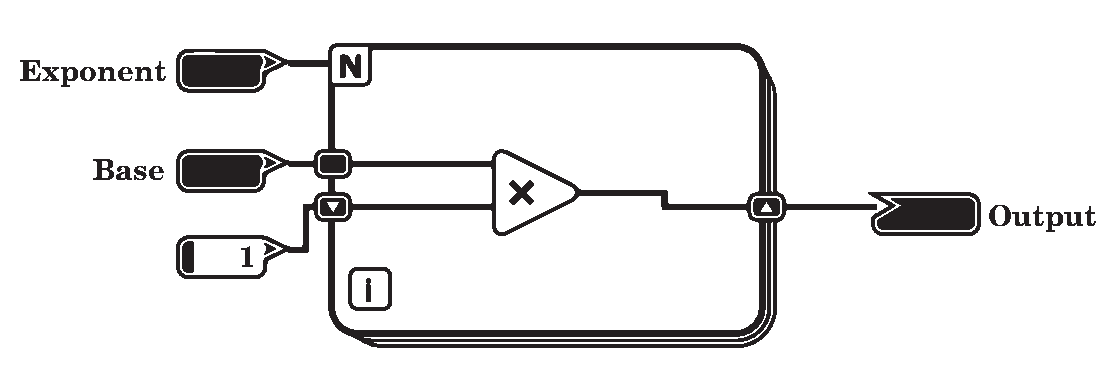
\includegraphics[width=150mm,keepaspectratio]{figures/vi2.pdf}
\caption{Exponent function in G Language} 
\label{fig:gexponent}
\end{figure}

\subsubsection{Dataflow paradigm}
Execution of G programs differ from usual, sequential programs. The execution order of program statements is not defined, a statement (or node in LabVIEW) can be executed when all the inputs for a statement are ready. This brings parallelism into the language, but execution will be serial - LabVIEW software will usually run on hardware with single-core processor, and G code is compiled to machine code. \cite{labview_under_the_hood} The execution order of parallel nodes in not deterministic. 
\subsubsection{Built-in nodes}
The built-in LabVIEW nodes, or primitives are the basic building blocks of a LabVIEW program, that are not written in G language (so they are not subVIs), and they can be created from the tool box of the block diagram editor.

The primitives are grouped in the following categories (in the NXG version):
\begin{enumerate}
   \item \textbf{Program flow:} this category contains the essential control structures, like case or loop diagrams or event handlers
   \item \textbf{Data types:} the manipulation commands for each data type (Numeric, String, Array, Cluster, etc.)
   \item \textbf{Math:} from basic math operations (arithmetic, comparison) to advanced mathematics (linear algebra or integrals)
      \item \textbf{Analysis:} useful, optimized algorithms for signal processing and control applications
      \item \textbf{Hardware interfaces:} communication with external devices
            \item \textbf{Data communication:} communication inside the LabVIEW program, or over network
                  \item \textbf{Storage:} interface to the file system, or other storage
                        \item \textbf{User interface:} display dialogs or other GUI elements
         \item \textbf{Interop:} run C code or G code of other LabVIEW version, call system shell
\end{enumerate}

\subsubsection{An example block diagram}

%%%%%%%%%%%%%%


\subsection{Front panel}
Front panel is the user interface of a VI. It holds similar controls and indicators as a desktop forms application, such as input boxes, buttons, progress bars; as well as controls specific for engineering applications, like graphs, charts and waveform displays. Controls and indicators are  created automatically for a control or indicator node on the block diagram, and their values are linked. 

\begin{figure}
\centering
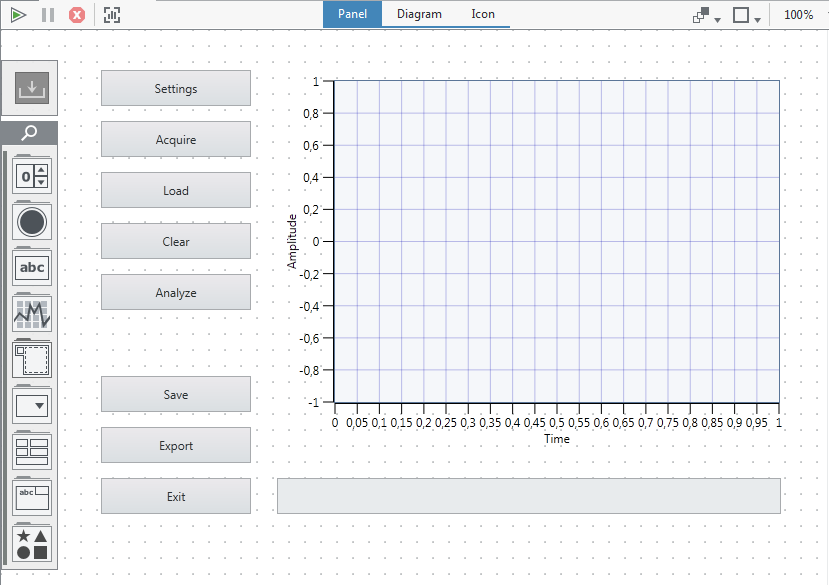
\includegraphics[width=120mm,keepaspectratio]{figures/frontpanel.png}
\caption{Front panel editor of a LabVIEW NXG measurement example} 
\label{fig:frontpanel}
\end{figure}

This way, all VIs can be run on their own (for instance, to manually test them), but in a large project VIs are hierarchically called, and usually there is a top VI, which is meant to be run. The VI also has an icon editor, to customize appearance as a subVI (with G being a graphical language, this is essential to maintain code readability). 
\subsection{Environment and hardware}
LabVIEW features an integrated development environment, which is intuitive to use for those who are familiar with other IDEs. The project structure is managed in the Project Explorer, where source code can be organized into folders and by targets. The VI Editor has two main views: one for the Front Panel, and one for the Block Diagram. Both views are graphical: the elements are placed from a toolbox with a drag and drop method. Running a VI is possible from both the VI Editor and the Project Explorer. For debugging, LabVIEW offers the Highlight Execution feature, which will slow down the execution of the VI and show the actual values of the wires on the block diagram.

After installing the necessary drivers, LabVIEW connects to NI hardware with minimal configuration, which can be performed with a tool called Measurement \& Automation Explorer (MAX), bundled with LabVIEW. These include data acquisition and control hardware (sensors, motion controls, displays), test and instrumentation hardware (oscilloscopes, multimeters, waveform generators), wireless hardware (spectrum and signal analysers, software defined radios). They can be accessed and controlled from LabVIEW directly.



%----------------------------------------------------------------------------
\chapter{Testing in LabVIEW}
%----------------------------------------------------------------------------

%\section{Testing measurement and control systems}
\section{Unit testing LabVIEW applications}
Unit testing in LabVIEW programs are commonly used in medium or large size projects, or where requirements are changing. Though, it is not a common practice everywhere, even if the project is an industrial application, where a fault is really expensive to recover. The main reason is to cut testing costs.

The testing techniques are similar to those in traditional programming languages, with a few differences. Software units can be a single VI, a group of VIs, or a LabVIEW class. Unit tests follow the xUnit schema: the tested unit gets pre-defined input sets, and the results are compared to the pre-defined outputs.

It is important to write testable code, that can run isolated from external dependencies, and does not require to run the entire program. "Spaghetti code", that is not able to run on its own, is not only bad from the perspective of testing, but can cause other problems (like re-usability in other projects, or maintaining compatibility with new versions of other components). In LabVIEW, it is really easy to fall in this trap, but following development guidelines help to evade it. Following Test Driven Development is also possible in LabVIEW, with nearly the same rules as in other languages - when the interface of a unit is defined, creating tests can begin \cite{delacor_ni2014}. 

There are really few unit testing tools and frameworks for LabVIEW compared to other languages\footnote{\url{https://en.wikipedia.org/wiki/List_of_unit_testing_frameworks}}, and they only support current generation LabVIEW (LV 2018), and not NXG.
\subsection{Self-made test fixtures}
It is always an option to build a test fixture manually (and in NXG it is the only option currently). Every test suite will get a harness VI, which executes several test cases. Test cases of a test suite will do the same action on the unit, but with several different input sets. The inputs and expected outputs can be defined in an array, a cluster, or other data structure, and then a loop iterates over the test cases, executing the VI under test for each set of parameters. The test verifies output values and error output if it is present. Setup and teardown parts can be included in the loop too (or global setup and teardown outside the loop), to initialize and prepare the unit, and to do any cleanup task necessary. A boolean output will indicate, whether the test suite passed or failed - in order to pass, all test cases must pass. The block diagram of an example test fixture is shown on Figure~\ref{fig:selfmadetestfixture}.
A top module is recommended, which contains all the Harness VIs, and summarizes the results. This could substitute the interface of a unit testing framework. 

\begin{figure}
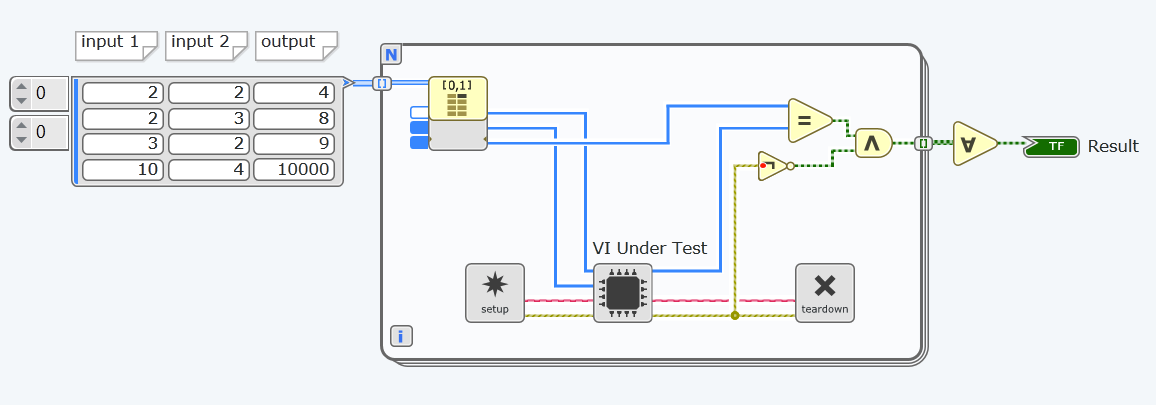
\includegraphics[width=150mm,keepaspectratio]{figures/lv_testsuite.png}
\caption{A test fixture in LabVIEW NXG} 
\label{fig:selfmadetestfixture}
\end{figure}

\subsection{Unit Test Framework}
Unit Test Framework\footnote{\url{http://sine.ni.com/nips/cds/view/p/lang/hu/nid/209043}} (or UTF for short) is the official unit testing tool for LabVIEW, released by National Instruments. It is available for purchase as an addon from LabVIEW Tools Network. UTF is the most popular unit testing framework, since it is covered by the support of National Instruments, an ISO certified company.

The interface of UTF is really easy to use, a unit test can be made in a few minutes. Test suites are stored in .lvtest files, which can be edited with a configuration panel. A tabular-style interface is used to define the inputs and outputs for each test case. Setup and teardown VIs, and other options can also be defined. There are a few special cases, when the desired behaviour cannot be expressed using the editor (like passing parameters to a teardown VI).

The results are shown in a dialog with other metrics, like code coverage. Status of the tests are shown also in the Project Explorer, for a quick check. UTF has the advantage to run tests on real-time NI hardware, like the CompactRIO\footnote{\url{http://www.ni.com/en-us/shop/compactrio.html}} \cite{labview_utf}. 
\subsection{JKI VI Tester}
VI Tester\footnote{\url{http://sine.ni.com/nips/cds/view/p/lang/hu/nid/215910}} is an open source tool from JKI Software. Based on the xUnit test achitecture, it is a really powerful test framework, that supports testing object-oriented LabVIEW programs well. Tests are created from a template, and organized into a test class. Assertion and other utilities can be used as a testing element subVI, as seen on Figure \ref{fig:vitester}. \cite{vitesterwiki}
\begin{figure}
\centering
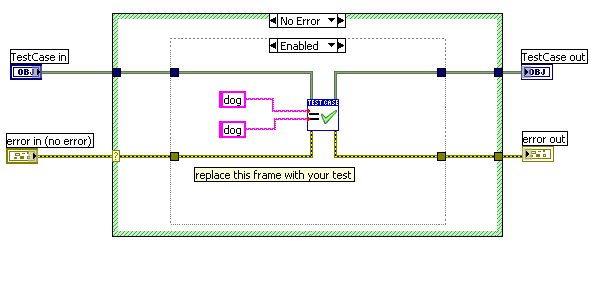
\includegraphics[width=120mm,keepaspectratio]{figures/vitester.png}
\caption{Example VI with an assertion} 
\label{fig:vitester}
\end{figure}
\subsection{Caraya}
Another unit test framework from JKI Software is Caraya\footnote{url{http://sine.ni.com/nips/cds/view/p/lang/hu/nid/215909}}, which uses a different approach. The main feature is the assertion subVI, which can be used on its own (outside a unit test), to ensure validity of data in a system in production. Tests are defined with Test Suite and Define Test subVIs, and unit tests defined like that get summarized in an interface like in JKI VI Tester \cite{carayapages}. 
\subsection{InstaCoverage}
InstaCoverage\footnote{\url{http://sine.ni.com/nips/cds/view/p/lang/hu/nid/216652}} is a new, xUnit-style tool. The test suites are stored in a similar way to UTF, but each test gets a harness VI, like in JKI's tools. Harness VIs are really minimalistic, therefore test execution is really quick. InstaCoverage tests can also run on real-time hardware \cite{icovsite}. 
%----------------------------------------------------------------------------
\chapter{Design}
%----------------------------------------------------------------------------
\section{Goals}
My goal is to implement a tool in LabVIEW, which can provide test inputs for a single VI, its front panel controls or input terminals. These test inputs should cover all the possible execution paths (in the case of LabVIEW, all the subdiagrams, or all combination of subdiagrams). After running the tool, outputs for each input set can be easily defined executing the VI. A tool like this can later help with unit test generation: using the generated input and output sets, xUnit-style tests can be created automatically, which will have 100\% branch (diagram) coverage.

According to my knowledge, no such tool exists for LabVIEW yet, so a simple tool created for the BSc thesis can be later be improved and used in an automatic test generation project.

A possible solution is symbolic execution of the VI: defining the input controls (data accessors) as symbolic variables, the constraint solver will try to determine the values in all the execution tree leafs.
\section{Scope}
During this BSc thesis, I am going to implement a prototype tool with basic functionality, and with support for a limited set of LabVIEW elements. This tool can later be improved, adding the whole set of LabVIEW primitives, and possibly developed into a whole test generation solution. 

Requirements for the prototype:
\begin{enumerate}
\item Return all possible paths (and path conditions) for VIs that have one or more case structures (with boolean conditions)
\item Specify input variables to be used to reach a path
\item Return only one path for VIs without a case structure
\item Support basic arithmetical, comparison and logical operations (+, -, *, ++, --, <, >, ==, And, Or, Not) during execution
\item Support integer an boolean data types
\item Stop execution of paths with an unsatisfiable condition
\end{enumerate}

\section{Architecture}

The tool will be a plugin of LabVIEW NXG, to have access to the programming interface and object model of VIs, and to integrate the tool to the UI. The tool will use the Z3 Solver too, referenced as a library.

Two main parts of the tool will be the Parser and the Symbolic Execution Loop. The job of the parser is to interpret and convert a LabVIEW VI into a form that can be later used during symbolic execution. The second part, Symbolic Execution Loop iterates through the converted procedural program, executing the statements, and forking when necessary. The output of the program is an execution tree, with its leafs associated to the possible execution paths of the program. These leafs will contain a path condition, which can be evaluated by the Z3 Solver, returning input values to be used to reach that path.
\begin{figure}
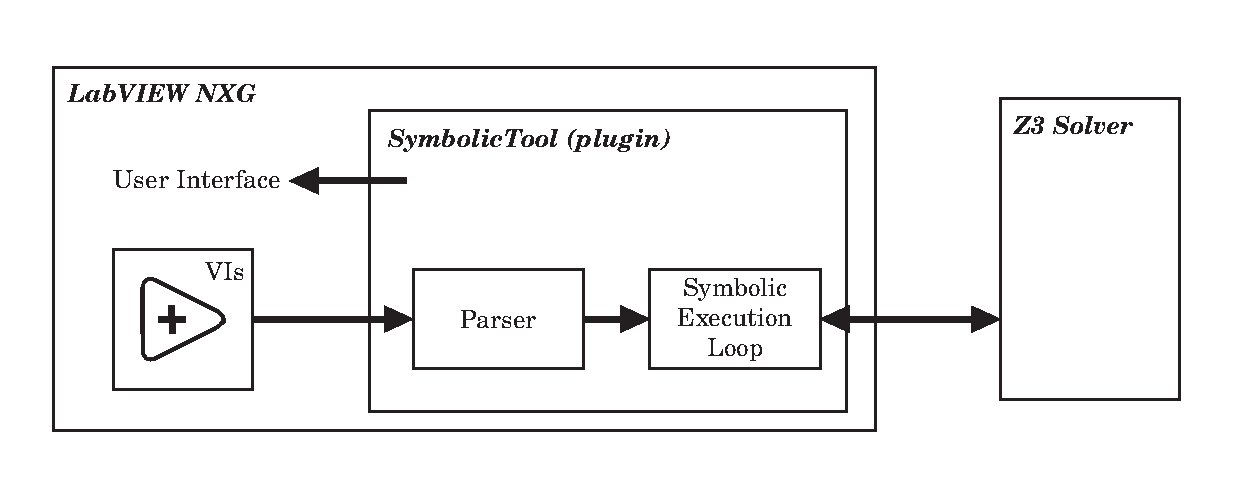
\includegraphics[width=150mm,keepaspectratio]{figures/architecture.pdf}
\caption{Architecture plan} 
\label{fig:architectureplan}
\end{figure}


The steps executed by the tool will be the following:

\begin{itemize}
  \item Access the object model of the tested Virtual Instrument
  \item Generate a procedural representation of the dataflow program (Parser)
  \item Execute the procedural program with the inputs of the VI as symbolic variables (Symbolic Execution Loop)
   \item Use a constraint solver to calculate the symbolic variables
in the leafs of the symbolic tree
     \item Display the calculated inputs (or use them to build a unit test)
  \end{itemize}

The first step depends entirely on the programming interface of NI software, so it will be a topic of the implementation section. Once the data model of the VI is accessible, it can be converted to a procedural program. To do this, an object model for the program has to be designed, which is tailored for the purpose of symbolic execution.

\section{Getting the program ready for symbolic execution}

The topic of symbolic execution is well defined in the area of procedural programming, but not for dataflow programming.

\begin{figure}
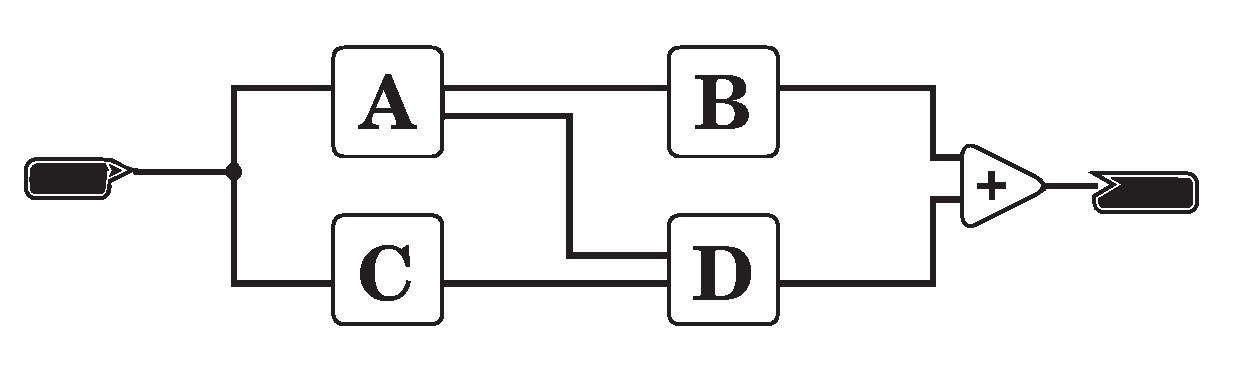
\includegraphics[width=150mm,keepaspectratio]{figures/vi1.pdf}
\caption{Dataflow program example} 
\label{fig:dataflowexample}
\end{figure}

\begin{lstlisting}[frame=single,float=!ht,caption={The same program using a procedural paradigm},captionpos=b,label={lst:proceduralexample},language=]
IN: i
(w1,w2) = A(i)
w3 = B(w1)
w4 = C(i)
w5 = D(w2,w4)
o = w3 + w5
OUT: o
\end{lstlisting}

I decided to convert the dataflow program to a procedural one, this means to define the execution order of nodes and turning the data flow wires into variables. This is possible, since executing a program in LabVIEW does the same - when running on the computer, the nodes execute in some order after each other. A node can execute, when all the input values are ready. This can also be observed in the development environment using the Highlight Execution tool, after executing a node the output values will slowly move to the next node. A G program cannot contain a wire cycle (except with feedback nodes), thus the nodes form a directed acyclic graph, which will have a topological ordering. When two or more topological ordering exist, it may be worth to choose the one that has forking statements later in the execution, to reduce execution time. Control structures will be quite easy to handle: case structures and loops are subdiagrams on a VI, and during conversion the contents of subdiagrams will become parts of If-Else statements and While loops. 
\section{Symbolic execution of a VI}

If performed correctly, the conversion will produce a simple algorithmic representation of the dataflow program. Symbolic execution can now be run.

From the symbolic execution point of view, VIs (Virtual Instruments) can be treated as the program, on which the symbolic execution is done. It has inputs, outputs, and most of the instructions are usually the native components of LabVIEW (so that their behaviour can be predicted). Controls are going to be the inputs, their data type can be chosen as one of the basic types, clusters (similar to struct), or objects. In the case of the symbolic execution tool, I am going to stick to the basic types. Indicators are the outputs of the program.

Instruction blocks use wires to pass data to each other. They are similar to variables in text-based languages, but they also define order of execution between blocks. Since each wire is going to represent a new variable in the program, the symbolic executor will have to deal with lots of unnamed variables.

Another issue is dealing with nodes that depend on external data source, or those that perform an operation that is not supported by the constraint solver.

\subsection{Program flow elements}
For loop, while loop and case structure are the basic building blocks of any program. Converting them from dataflow is straightforward, and symbolic execution is defined for those. If having loops in the program, with a symbolic condition, a maximum depth of execution tree has to be defined, not to get stuck with an infinite number of iterations. Feedback nodes and shift registers inside loops behave like variables, passing values from one iteration to the next.

Sequence and disable structures are only involved during the conversion: sequence structure defines order of execution, which the converted program will naturally has; disabled parts will be simply ignored (or treated like a case structure, based on preference). Event structures are hard to deal with, an event can be raised any time during execution. If no other task runs parallel to the event loop, they can be best represented with a case structure for all possible events, with a symbolic variable as its input, inside a loop.

Timing blocks will simply be ignored, as they are irrelevant to symbolic execution. 

In the first prototype of the tool, I decided to implement the Case Structure only, this is the element, on which it is the easiest to demonstrate symbolic operation. 
\subsection{Arithmetic, logic, and other operations}
Basic arithmetical and logical operations, like addition, subtraction are easy to implement and to be solved by the constraint solver. Multiplication and division are also easy to implement, but can create such a nonlinear problem, that the solver cannot calculate. 

More complex operations, like trigonometric functions and signal processing can be approximated with a constant value or linear function. External dependencies, like storage or network access are black box - they can be substituted with an expected value, or another symbolic variable.

In the prototype, basic arithmetic and logic will be implemented.

\subsection{Object model}

The starting point of the model will be the class \textit{Statement}, which is the same unit in the program as a node in the VI. These \textit{Statement}s will execute in a defined order, which is managed by a \textit{Sequence} object. \textit{Sequence} corresponds to the Block Diagram of the VI, or any subdiagram (in a case structure or a loop). Since a Node in the VI can do complex tasks, and have multiple outputs, a \textit{Statement} can be broken down to simpe instructions, \textit{Assignment}s, that evaluate an \textit{Expression}, and place the result in a \textit{Variable}.

\textit{Expression} is just an empty base class for the expression classes to derive from. This approach provides extensibility, any kind of expression can be treated the same way, and with the help of \textit{Operators}, complex expressions with two or more levels can be built.

\textit{IfStatement} and \textit{LoopStatement} will have \textit{Statement} as their ancestor to be able to join a \textit{Sequence}. The subdiagrams of a case structure or a loop will be a part of these \textit{Statement}s as \textit{Sequence}s.
\begin{figure}

\centering
\begin{tikzpicture}[node distance = 1cm, auto]
    % Place nodes
   
    
    \node [block] (seq) {Sequence};
    \node [block, below=of seq] (statement) {Statement};
    \node [block, below=of statement] (ifs) {IfStatement};
    \node [block, below right=of statement] (loop) {LoopStatement};
        
    \node [block, below left=of statement] (assignment) {Assignment};
    \node [block, below=of assignment] (expression) {Expression};
    \node [block, below left=of expression] (variable) {Variable};
    \node [block, below=of expression] (symvar) {SymbolicVar};
    \node [block, below right=of expression] (oper) {Operator};
    \node [block, right=of oper] (const) {Constant};
        
    \path [comp] (statement) -- (seq);
    \path [comp] (assignment) |- (statement);
     \path [generalization] (ifs) -- (statement);
     \path [generalization] (loop) |- (statement);
     \path [aggr] (expression) -- (assignment);
          \path [aggr] (variable) |- (assignment);
               
     \path [generalization] (variable) |- (expression);
     \path [generalization] (symvar) -- (expression);
     \path [generalization] (oper) |- (expression);
     \path [generalization] (const) |- (expression);
               
   % \node [block, below right=1cm and -2.6cm of arch] (des) {Detailed design};
    % \node [block_rounded, below right=1cm and -1cm of des] (dev) {Development};
  %  \node [block_rounded, above right=1cm and -1cm of dev] (utest) {Build and unit test};
 %   \node [block_rounded, above right=1cm and -2.6cm of utest] (itest) {System integration and test};
  %  \node [block_rounded, above right=1cm and -2.6cm of itest] (dep) {Deployment and verification};
    % Draw edges
 %   \path [line] (req) -- (arch);
  %  \path [line] (arch) --  (des);
  %  \path [line] (des) -- (dev);
  %  \path [generalization] (dev) -- (utest);
 %   \path [comp] (utest) -- (itest);
  %  \path [line] (itest) -- (dep);
  %  \path [double] (des) -- (utest);
   % \path [double] (arch) -- (itest);
   % \path [double] (req) -- (dep);
    
\end{tikzpicture}

\caption{Simplified diagram of the procedural program data model} 
\label{fig:datamodeldiagram}
\end{figure}



\section{Limitations}
%----------------------------------------------------------------------------
\chapter{Implementation}
%----------------------------------------------------------------------------
\section{Different versions of NI LabVIEW}
At the time of writing this thesis, National Instruments offers two versions of LabVIEW: LabVIEW 2018\footnote{\url{http://www.ni.com/en-us/shop/labview/labview-details.html}}, and LabVIEW NXG\footnote{\url{http://www.ni.com/en-us/shop/labview/labview-nxg.html}}. LabVIEW 2018 is a sequel to the LabVIEW versions released in the past few years, it operates reliably and fast, has support for all the NI hardware, and has a wide range of features. LabVIEW NXG is a brand new product, it has been created from scratch, and has been developed according to current standards - optimized for the newest hardware and software, and a really comfortable UI. Most features are still beta however, or under development\footnote{\url{http://www.ni.com/pdf/products/us/labview-roadmap.pdf}}, a large number of hardware are not yet supported, and the operation is not as reliable as the current generation software.\cite{nxg_article}

LabVIEW 2018 and LabVIEW NXG are not really compatible with each other, though the interface and the programming is similar, they have completely different execution engines and file formats. There is a tool bundled with NXG for current generation project conversion, but it is not perfect, and almost always the converted VIs need manual fixing afterwards.

Given two distinct LabVIEW products, it has to be decided which to develop the tool for. Both of them have advantages: current generation LabVIEW has a larger user base than NXG, but developing for NXG will make the tool compatible with actual software for a longer time (since NXG will eventually replace current generation LabVIEW).
\subsection{Comparing the API}
For making a decision on the LabVIEW version, the main point was the method of integrating the tool into LabVIEW. 

Reading the VI data from file is quite difficult. The file format definition of current generation VIs is not published, so the only software that can read the file is LabVIEW. NXG stores the VI data in XML files, which is a lot friendlier. It is possible to create an interpreter, and build the object model, since the nodes are XML elements, and the connections are made using unique identifiers.

Building a plugin is an option too. LabVIEW 2018 has a toolbox called VI Scripting\footnote{\url{http://sine.ni.com/nips/cds/view/p/lang/en/nid/209110}} for G language. It has several commands to access or modify VI object models and project structure. Project Provider Framework\footnote{\url{http://www.ni.com/white-paper/13921/en/}} allows an add-on to be integrated into the interface of LabVIEW, like creating a menu command or a toolbar button.

A plugin for LabVIEW NXG needs a different approach. Most of NXG uses .NET framework, and an add-on integrates in a form of a .NET class library (DLL). The object model of a Virtual Instrument is directly accessible as a .NET object, and plugin entry points can easily be defined with class attributes. UI elements can be easily created as well. This way, the plugin is written in C\# language.

I have chosen to create an NXG plugin, since writing such a complex tool in G language would require such an expertise in LabVIEW, that I do not have. Additionally, I already had the routine in NXG API and C\#.
\section{LabVIEW NXG API and object model}
There is hardly any documentation on the NXG programming interface at the moment, but an example plugin project on GitHub\footnote{\url{https://github.com/ni/nidevlabs}}. Fortunately, this project had almost all the API I needed for this project.
\lstset{escapechar=@}
\begin{lstlisting}[frame=single,escapechar=@,float=!ht,caption={NXG plugin entry point},captionpos=b,label={lst:menuapi},language=C++]
[ExportPushCommandContent]
public class LauncherCommands : PushCommandContent
{
    public static readonly ICommandEx SymbolicMenuRoot = new RelayCommandEx(RelayCommandEx.HandleNoOp)
    {
        UniqueId = "SymbolicTool.MenuRoot",
        LabelTitle = "SymbolicTool",
        MenuParent = MenuPathCommands.RootMenu
    };
    public readonly ICommandEx RunCommand = new ShellRelayCommand(OnRun)
    {
        UniqueId = "SymbolicTool.RunCommand",
        LabelTitle = "Run Symbolic Execution",
        MenuParent = SymbolicMenuRoot
    };
    public override void CreateApplicationContent(ICommandPresentationContext context)
    {
        base.CreateApplicationContent(context);
        context.Add(SymbolicMenuRoot);
        context.Add(RunCommand);
    }
    public static void OnRun(ICommandParameter parameter, ICompositionHost host, DocumentEditSite site)
    {
        // Run the program here
    }
}
\end{lstlisting}

\begin{figure}

\centering
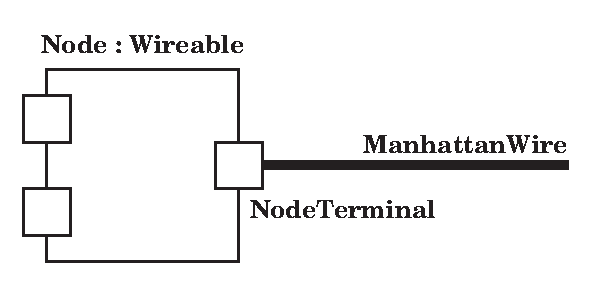
\includegraphics[width=80mm,keepaspectratio]{figures/lvobject.pdf}
\caption{LabVIEW Node object model} 
\label{fig:lvobject}
\end{figure}
I implemented a launcher code based on the ExamplePlugins project, that integrates a menu command into the menu bar of NXG (Listing \ref{lst:menuapi}). The three parameters of the callback function provide access to the object model of LabVIEW. DocumentEditSite refers to the currently opened document, and since the execution will run on the opened VI, getting the model will be really easy: \lstinline[columns=fixed]{rootElement = site.ActiveDocumentEditor?.EditorInfo?.RootElement;}. The model will be passed to the parser component, then the returned Sequence object (which holds the procedural program) is given to the symbolic execution module (Listing \ref{lst:launchercode}). When finished, values of symbolic variables will be placed in each leaf, and can be retrieved using a \lstinline[columns=fixed]{leaf.getSymbols()} call.
\lstset{escapechar=@}
\begin{lstlisting}[frame=single,escapechar=@,float=!ht,caption={Launcher code},captionpos=b,label={lst:launchercode},language=C++]
public static void OnRun(ICommandParameter parameter, ICompositionHost host, DocumentEditSite site)
{
    var rootElement = site.ActiveDocumentEditor?.EditorInfo?.RootElement;
    if (rootElement == null) return;
    var sequence = VIConverter.VIConverter.CreateModel(rootElement);
    Symbolic.SymbolicExec se = new Symbolic.SymbolicExec(sequence.getStatements());
    List<Symbolic.ExecutionState> leafs = se.Execute();
    // Print symbolic variable values
}
\end{lstlisting}
\section{The parser}
The algorithm used in the main parser loop is a sort of breadth-first search. The nodes waiting to be processed get placed in a queue object (which initializes with those nodes, that have no input wires, and can be executed right away). The main loop takes a node from the front of the queue, and makes sure all its input nodes are already processed - this is important, because at the end of processing a node, all the output nodes are added to the queue, and they not necessarily have all their inputs ready. 

A \textit{Statement}\footnote{Note: the classes of my implementation are indicated with \textit{italic}, the classes of LabVIEW API are indicated with \underline{underlined} font} is created for the node, then the arithmetical, logical or other operations are added respectively: an \textit{Expression} (which can be as simple as an addition, or a more complex expression, a nested structure of \textit{Operator}s) placed in an \textit{Assignment}, which assigns the \textit{Expression} value to a \textit{Variable}. When the node is a \underline{DataAccessor} (LabVIEW control), a \textit{SymbolicVariable} will be introduced.


\begin{algorithm}
\ForEach{nodes of rootElement without input wires}{
add node to nextNodes\;
}
\If{rootElement is NestedDiagram}{
\ForEach{input tunnels}{
add output nodes to nextNodes\;
}
}
\While{nextNodes is not empty}{
thisNode:=nextNodes.Dequeue\;
\eIf{thisNode has all inputs ready}{
statement:=new Statement\;
inputVariables:=variableDictionary[input wires of thisNode]\;
\ForEach{output wires of thisNode}{
variableDictionary[output wire]:=new Variable\;
}
\Switch{type of thisNode}{
\uCase{SourceModel.Add}{statement.addOperation(createAssignment(outputVariables[0], createAddition(inputVariables[0], inputVariables[1])))\;}
\uCase{SourceModel.Multiply}{statement.addOperation(createAssignment(outputVariables[0], createMultiplication(inputVariables[0], inputVariables[1])))\;}
\vspace{2mm}
...\\
\uCase{SourceModel.Literal}{statement.addOperation(createAssignment(outputVariables[0], createConstant(thisNode.Data)))\;}
\uCase{SourceModel.DataAccessor}{statement.addOperation(createAssignment(outputVariables[0], createSymbolicVariable(thisNode.DataItemName)))\;}
\Case{SourceModel.BorderNode}{
\If{thisNode.Owner is CaseStructure and all its inputs are ready}{
create variables for all input and output tunnels\;
statement:=new IfStatement\;
statement.trueBranch:=Parser(true diagram)\;
statement.falseBranch:=Parser(false diagram)\;

}
}
}
sequence.add(statement)\;
\ForEach{follow output wires of thisNode}{
nextNodes.Enqueue(found node)\;
}
}{
nextNodes.Enqueue(thisNode)\;
}

}
 \caption{A simplified algorithm of Parser(rootElement)}
 \label{alg:parser}
\end{algorithm}

The parser binds a \textit{Variable} to all of the wires. New \textit{Variable}s are introduced, when the parser processes the output wires of a node (since a wire can be connected to only one node output), and all \underline{ManhattanWire} - \textit{Variable} pairs will be stored in a lookup table (C\# Dictionary) global to a single run of the algorithm. This way, if multiple nodes use that output as an input, it will be the same \textit{Variable}.

When the search reaches a case structure, the parser will be recursively called for both subdiagrams. Wires enter the case diagram through \underline{BorderNode}s (or tunnels), so that for each of them a new \textit{Variable} will be introduced. In a subdiagram, the search will start from the \underline{BorderNode}s (and the nodes without input wires). After the search execution for both diagrams, the execution returns to the root parser.

To summarize, the simplified pseudo-code is listed in Algorithm \ref{alg:parser}, that is easier to understand than the original source. 
The explanation of data structures used during the operation of the parser:

\begin{itemize}
\item \textbf{rootElement} : \underline{Element} -- the parameter of the algorithm, the diagram, whose immediate child nodes must be searched
\item \textbf{nextNodes} : Queue<\underline{Wireable}> -- found \underline{Nodes}, waiting to be processed
\item \textbf{variableDictionary} : Dictionary<\underline{ManhattanWire}, \textit{Variable}> -- association between LabVIEW wires and variables in the procedural program
\item \textbf{sequence} : \textit{Sequence} -- the procedural program, chain of \textit{Statement}s, the result of this algorithm
\end{itemize}



Of course, this pseudo-code is more of a demonstration, than the actual program. A number of workaround solutions had to be used to handle special cases in the block diagram. For instance, when a case structure had two output tunnels, that connect to one source in the subdiagram, two variables were created for the same wire, which is invalid. The second variable had to be assigned the value of the first variable.

Since references from one LabVIEW object to another were mostly using a heterogenous collection, type checks and type casts take up a large percentage of the source code.

\section{Symbolic Execution Loop}

As mentioned earlier, symbolic execution is an extension to regular execution. The loop will iterate through the program, and execute the statements as it would normally, if there are no symbolic variables present.

The current execution environment is stored in an \textit{ExecutionState} object. This object stores the calculated values of \textit{Variable}s and the path condition throughout the execution. If the value of a variable is calculated from a symbolic variable, an \textit{Expression} containing the \textit{SymbolicVar} gets stored. It is important, that these values never store a reference to another \textit{Variable} object, when evaluating such an expression, since these might change after assignment, and the values would become invalid. During evaluation, the stored value of the \textit{Variable} is substituted into the expression, and if the two operands of an \textit{Operator} are constant values, the corresponding operator can evaluate with their values (see Listings \ref{lst:operator_eval} and \ref{lst:variable_eval}). 

\begin{lstlisting}[frame=single,escapechar=@,float=!ht,caption={Evaluation part of the Operator class},captionpos=b,label={lst:operator_eval},language=C++]
class Operator : Expression
{
    Expression A { get; set; }
    Expression B { get; set; }
    string Op { get; set; }
    
    // ...
    
    public override Expression Evaluate(ExecutionState es)
    {
        Expression a = A.Evaluate(es);
        Expression b = null; // for expressions with only one operand
        if (B!=null)b = B.Evaluate(es);
        if (a is Constant && b is Constant)
        {
            switch (Op)
            {
                case "+":
                    return new Constant((a as Constant).Value + (b as Constant).Value);
                // ...
            }
        }
        // ...
        return new Operator(a, b, Op);
    }
}
\end{lstlisting}

\begin{lstlisting}[frame=single,escapechar=@,float=!ht,caption={Evaluation part of the Variable class},captionpos=b,label={lst:variable_eval},language=C++]
class Variable : Expression
{
    string Name { get; set; }

    // ...
    
    public override Expression Evaluate(ExecutionState es)
    {
        return es.GetVariableValue(this);
    }
}
\end{lstlisting}

\begin{lstlisting}[frame=single,escapechar=@,float=!ht,caption={The part of ExecutionState related to execution},captionpos=b,label={lst:executionstate},language=C++]
class ExecutionState
{
    public Dictionary<Variable, Expression> variableValues = new Dictionary<Variable, Expression>();
    public Expression Pc;

    // ...

    public Expression GetVariableValue(Variable v)
    {
        return variableValues[v];
    }
    public void SetVariableValue(Variable v, Expression e)
    {
        variableValues[v] = e;
    }
    public ExecutionState Clone()
    {
        return new ExecutionState(new Dictionary<SymbolicVar, Expr>(symbolicVariables), new Dictionary<Variable, Expression>(variableValues), Pc);
    }

    public ExecutionState(Dictionary<SymbolicVar, Expr> symbolicVariables, Dictionary<Variable, Expression> variableValues, Expression pc)
    {
        this.symbolicVariables = symbolicVariables;
        this.variableValues = variableValues;
        Pc = pc;
    }
    // ...
}

\end{lstlisting}

The interesting part is handling \textit{IfStatement}s. The true and false branches of the structure are stored in the object as \textit{Sequence}s, therefore a new execution can be started for each of them. 

Before doing that, it must be verified, if the path condition extended with the condition of the if statement (or its negate for the false branch) is satisfiable or not. (For doing that the constraint solver will already be used. It will be described in the later sections, how \textit{Expression}s are getting handed to the solver.) If it is satisfiable, the execution state gets cloned for each branch, and updated with the extended path conditions. 

At this point, the operation of the tool resembles a depth-first search algorithm: the execution of the two execution branches begin right away, one after another, and each gets the program sequence from their part of the if statement, plus the rest of the program after the if statement. This way, the remaining part of the program will run twice, in the context of both branches.

When the run comes to the end, the routine returns the \textit{ExecutionState} of the finished program. This \textit{ExecutionState} (possibly) gets returned to the evaluation to the if statement, where these states are added to a list, and after executing both branches, the routine returns with the list. 

It can be seen, that calling the symbolic execution routine on the sequence of the entire program will return a list of \textit{ExecutionState}s of all possible execution paths (these are the leafs of the execution tree). These all have their own path condition, which now can be evaluated by the solver, to get the input values for each of them.

\section{Running the solver}
At the end of execution, \textit{ExecutionState} objects will contain a path condition (\textit{Expression}), which consist of symbolic variables, constant values, and operators. These kind of formulas are the constraints, the solver is expecting, it just needs to be translated to its own language. 

The object model of the solver is really similar to the \textit{Expression} model used in the tool. All of the \textit{Expression} classes get a \lstinline[columns=fixed]{Microsoft.Z3.Expr BuildTerm(Context ctx, ExecutionState es);} function, which builds the Z3 expression recursively. The needed symbolic variables are defined during this conversion (and are stored in \textit{ExecutionState}, for not to redefine in the case of multiple usage). The relevant parts are listed in Listing \ref{lst:executionstate_solver}.


\begin{lstlisting}[frame=single,escapechar=@,float=!ht,caption={Calling the solver in ExecutionState},captionpos=b,label={lst:executionstate_solver},language=C++]
class ExecutionState
{
    // ...
    public Dictionary<SymbolicVar, Expr> symbolicVariables = new Dictionary<SymbolicVar, Expr>();
    // ...
    public Expression Pc;

    public Expr GetSymbolicVariable(SymbolicVar s, Context ctx, Sort range=null)
    {
        if (symbolicVariables.ContainsKey(s))
        {
            return symbolicVariables[s];
        }
        else
        {
            if (range == null) range = ctx.MkIntSort();
            Expr e = ctx.MkConst(s.Name, range);
            symbolicVariables.Add(s, e);
            return e;
        }
    }
    // ...
    private Solver GetSolver()
    {
        if (Pc == null) Pc = new BoolConstant(true);
        using (Context ctx = new Context())
        {
            symbolicVariables.Clear();
            Expr pathCondition = Pc.BuildTerm(ctx, this);
            Solver s = ctx.MkSolver();
            s.Assert((BoolExpr)pathCondition);
            return s;
        }
    }
    public bool CheckModel()
    {
        Solver s = GetSolver();
        return s.Check().ToString().Equals("SATISFIABLE");
    }
    public Dictionary<string, string> GetSymbols()
    {
        Dictionary<string, string> symbols = new Dictionary<string, string>();
        Solver s = GetSolver();
        var check = s.Check();
        Microsoft.Z3.Model m = s.Model;
        foreach(FuncDecl d in m.Decls)
        {
            symbols.Add(d.Name.ToString(), m.ConstInterp(d).ToString());
        }
        return symbols;
    }
}

\end{lstlisting}

\section{Displaying the output}
For this is only a prototype, the results, which are the list of execution paths, their path conditions, and the calculated symbolic variables. After getting the execution tree leafs (see Listing \ref{lst:launchercode}), a simple string builder loop collects the data from the output structures, and the final string gets displayed in a \underline{NIMessageBox}.
%----------------------------------------------------------------------------
\chapter{Evaluation}
%----------------------------------------------------------------------------
\section{Displaying the procedural program}
During development, and when running the finished tool, it became very important to see the output of the parser part in an easy to read form. The C\# debugger did not fit for that job, since despite that I could see the object hierarchy, and inspect values and statements one-by-one, I could not see the converted program as a whole. 

Therefore, I overrode the ToString functions for all the model objects to return an easy to read string reflecting its contents. After that, all I had to do was to call ToString on a \textit{Sequence} object, and it returned a pseudo-code of the converted program.

In the following examples, the shown converted procedural examples are the output of this routine.
\section{Small demos}
\paragraph{Demo "A"}
For the first demo I used the same program, which I used to demonstrate symbolic execution in the Background section (Listing \ref{lst:symbolic_test}). The dataflow counterpart of that program can be seen on Figure \ref{fig:testvi1}.
\begin{figure}
\centering
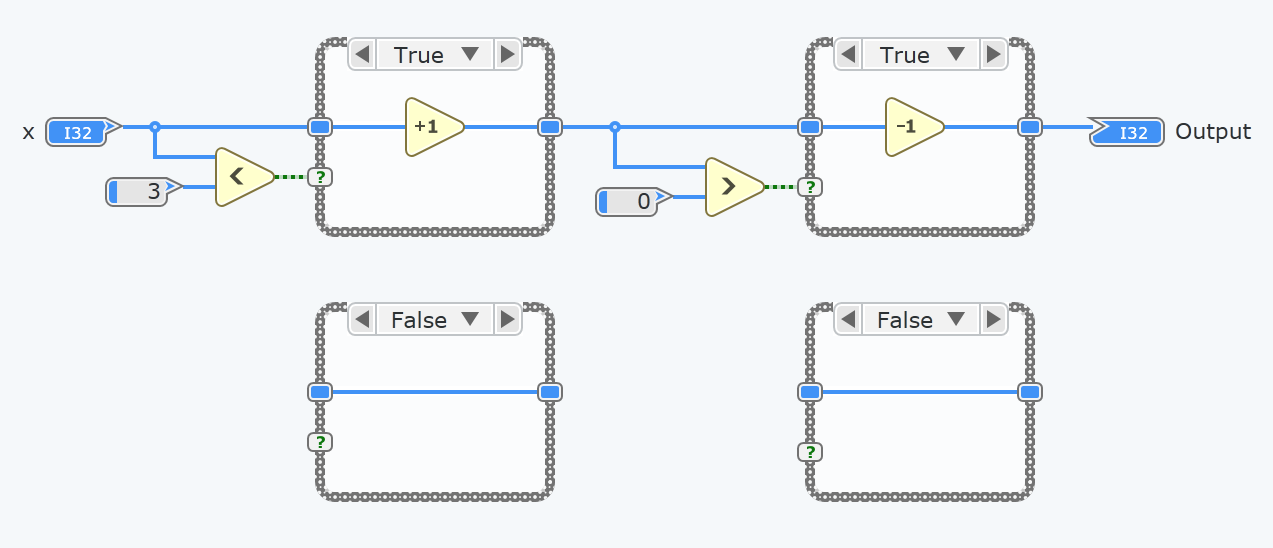
\includegraphics[width=150mm,keepaspectratio]{figures/testvi1.png}
\caption{Example VI "A"} 
\label{fig:testvi1}
\end{figure}

\begin{lstlisting}[frame=single,float=!ht,caption={The converted procedural version of VI "A"},captionpos=b,label={lst:testvi1_proc},language=]
A = [x]; 
B = 3; 
C = 0; 
D = (A < B); 
IF D Then
E = (A + 1); 
ELSE
E = A; 
End IF
F = (E > C); 
IF F Then
G = (E - 1); 
ELSE
G = E; 
End IF
[Output] : G; 
\end{lstlisting}

\begin{lstlisting}[frame=single,float=!ht,caption={The output of the symbolic execution for VI "A"},captionpos=b,label={lst:testvi1_sym},language=]
pc: (([x] < 3) & (([x] + 1) > 0)), x=0
pc: (([x] < 3) & !(([x] + 1) > 0)), x=-1
pc: (!([x] < 3) & ([x] > 0)), x=3
\end{lstlisting}

The outputs of symbolic execution in this example (Listing \ref{lst:testvi1_sym}) are the same as the expected (see Figure \ref{fig:symbolic_test}), and the unreachable fourth execution path $(!([x] < 3) \& !([x] > 0))$ is omitted from the list.

To verify the correctness of the results, I ran the VI with these inputs, to see if they really produce different execution paths. As seen on Figure \ref{fig:verify1}, all the possible paths have been covered with this input set.
\begin{figure}
\centering
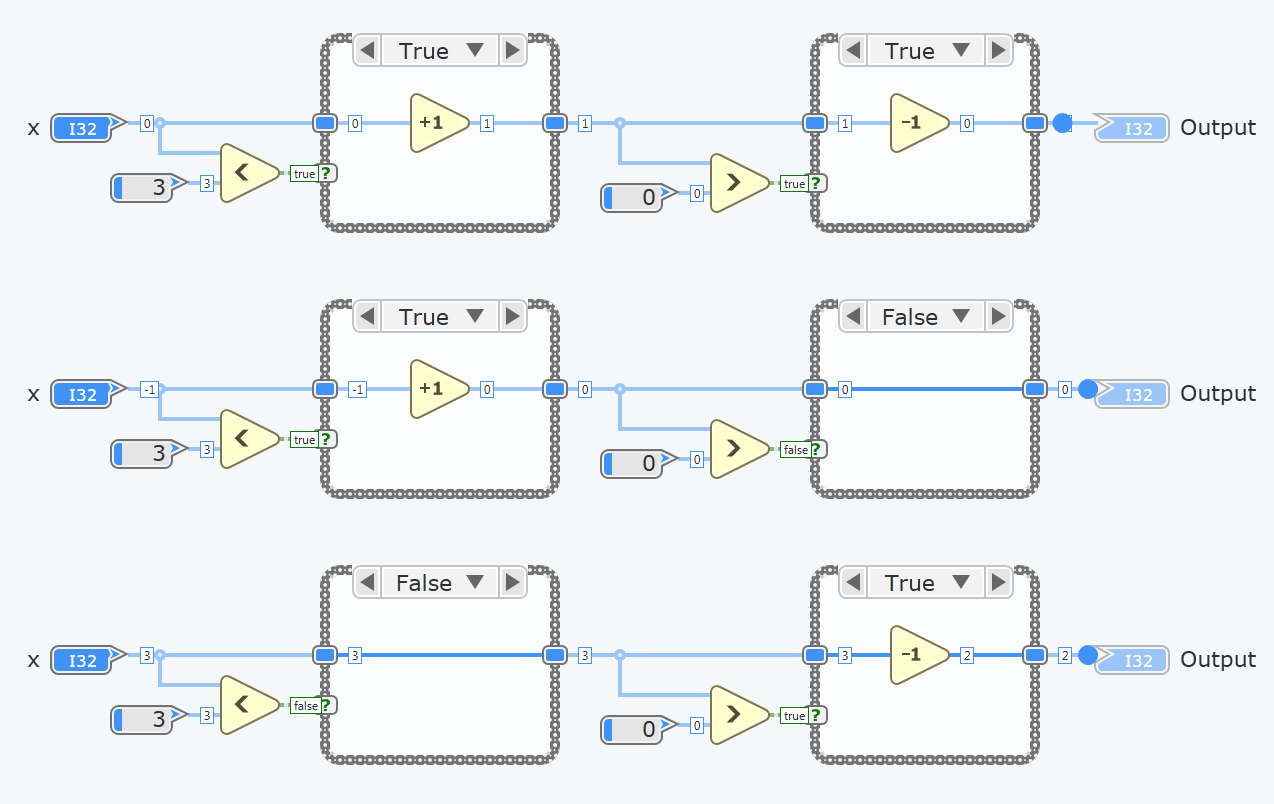
\includegraphics[width=140mm,keepaspectratio]{figures/verify1.png}
\caption{Run VI "A" with the result values as input} 
\label{fig:verify1}
\end{figure}

\paragraph{Demo "B"}
I wanted to test, if nesting case structures behaves correctly. When \textit{outside var} is false, \textit{inside var} should not matter in the path condition. Additionally, this test verifies, that boolean input values are processed correctly.

\begin{figure}
\centering
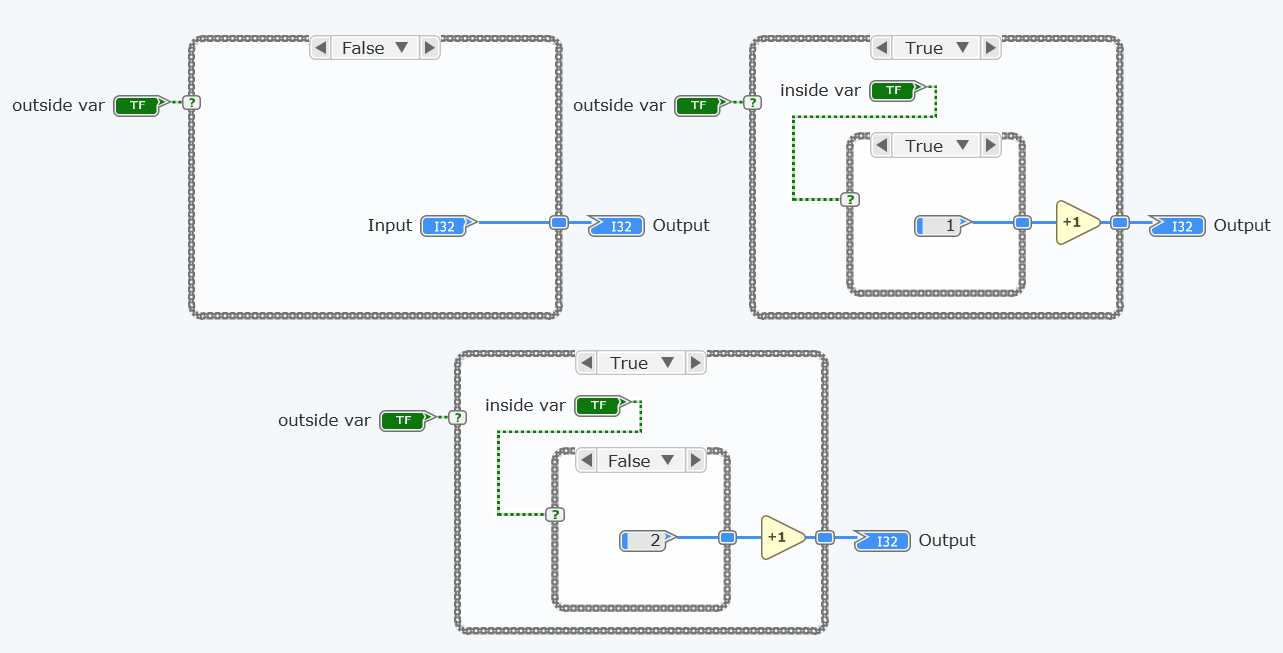
\includegraphics[width=150mm,keepaspectratio]{figures/testvi2.png}
\caption{Example VI "B"} 
\label{fig:testvi2}
\end{figure}


\begin{lstlisting}[frame=single,float=!ht,caption={The output of the symbolic execution for VI "B"},captionpos=b,label={lst:testvi1_sym},language=]
pc: ([outside var] & [inside var]), inside var=true, outside var=true
pc: ([outside var] & ![inside var]), inside var=false, outside var=true
pc: ![outside var], outside var=false
\end{lstlisting}

%% screenshots
%----------------------------------------------------------------------------
\chapter{Conclusion}
\label{chap:conclusion}
%----------------------------------------------------------------------------

In this semester, I learned about a new testing technique, symbolic execution, which is the foundation of most of the popular unit test generation frameworks -- it can specify test inputs, that will cover all (or most) execution paths of the program, making the test suite more complete. This method is powerful, but due to its resource-demanding nature it is quite difficult to implement correctly: running it on a large application without control can increase execution time exponentially. 

My prototype tool did not have to deal with this issue, but despite that, it was challenging to implement: the target platform was LabVIEW NXG by National Instruments, a system engineering tool, used by engineers worldwide. However, its dataflow-based graphical language is not the usual platform to perform symbolic execution on. I had to find a way to apply the technique of symbolic execution, which is well defined for imperative programs.

The solution was to implement a parser, which converts the dataflow program to an imperative one. That was the most difficult part of the implementation, because I had to get familiar with the object model (with almost no documentation), and there were a number of special cases that could be created in a LabVIEW program, which had to be handled with a workaround in the parser tool.

Based on the articles on symbolic execution, that part of the tool was quite easy to implement, especially because the data structure of the parsed program was nearly ideal to perform it. 

Although the finished prototype tool has a limited functionality, it might be a good starting point to develop an advanced test generation suite. No such tool exists for LabVIEW yet, therefore it would be a novelty tool, really useful to all the engineers using LabVIEW.


%\include{content/latex-tools}
%\include{content/thesis-format}
%\include{content/template-usage}


% Acknowledgements
%~~~~~~~~~~~~~~~~~~~~~~~~~~~~~~~~~~~~~~~~~~~~~~~~~~~~~~~~~~~~~~~~~~~~~~~~~~~~~~~~~~~~~~
%----------------------------------------------------------------------------
\chapter*{\koszonetnyilvanitas}\addcontentsline{toc}{chapter}{\koszonetnyilvanitas}
%----------------------------------------------------------------------------

%Ez nem kötelező, akár törölhető is. Ha a szerző szükségét érzi, itt lehet köszönetet nyilvánítani azoknak, akik hozzájárultak munkájukkal ahhoz, hogy a hallgató a szakdolgozatban vagy diplomamunkában leírt feladatokat sikeresen elvégezze. A konzulensnek való köszönetnyilvánítás sem kötelező, a konzulensnek hivatalosan is dolga, hogy a hallgatót konzultálja.

% ni trial
% szakmai gyakorlat labs

First of all, I wish to thank my advisor, Dr. Zoltán Micskei, for continuously helping my work on this BSc thesis. I would like to thank Dr. Péter Bokor and IncQuery Labs Ltd. for technical help and advice; National Instruments for providing me free trial of LabVIEW NXG. Finally, I wish to thank my family and my roommates for their support, they have been really an inspiration to me.


% List of Figures, Tables
%~~~~~~~~~~~~~~~~~~~~~~~~~~~~~~~~~~~~~~~~~~~~~~~~~~~~~~~~~~~~~~~~~~~~~~~~~~~~~~~~~~~~~~
%\listoffigures\addcontentsline{toc}{chapter}{\listfigurename}
%\listoftables\addcontentsline{toc}{chapter}{\listtablename}


% Bibliography
%~~~~~~~~~~~~~~~~~~~~~~~~~~~~~~~~~~~~~~~~~~~~~~~~~~~~~~~~~~~~~~~~~~~~~~~~~~~~~~~~~~~~~~
\addcontentsline{toc}{chapter}{\bibname}
\bibliography{bib/thesis}


% Appendix
%~~~~~~~~~~~~~~~~~~~~~~~~~~~~~~~~~~~~~~~~~~~~~~~~~~~~~~~~~~~~~~~~~~~~~~~~~~~~~~~~~~~~~~
%----------------------------------------------------------------------------
\appendix
%----------------------------------------------------------------------------
\chapter*{\fuggelek}\addcontentsline{toc}{chapter}{\fuggelek}
\setcounter{chapter}{\appendixnumber}
%\setcounter{equation}{0} % a fofejezet-szamlalo az angol ABC 6. betuje (F) lesz
\numberwithin{equation}{section}
\numberwithin{figure}{section}
\numberwithin{lstlisting}{section}
%\numberwithin{tabular}{section}

%----------------------------------------------------------------------------
%\section{A TeXstudio felülete}
%----------------------------------------------------------------------------
%\begin{figure}[!ht]
%\centering
%\includegraphics[width=150mm, keepaspectratio]{figures/TeXstudio.png}
%\caption{A TeXstudio \LaTeX-szerkesztő.} 
%\end{figure}

%----------------------------------------------------------------------------
%\clearpage\section{Válasz az ,,Élet, a világmindenség, meg minden'' kérdésére}
%----------------------------------------------------------------------------
%A Pitagorasz-tételből levezetve
%\begin{align}
%c^2=a^2+b^2=42.
%\end{align}
%A Faraday-indukciós törvényből levezetve
%\begin{align}
%\rot E=-\frac{dB}{dt}\hspace{1cm}\longrightarrow \hspace{1cm}
%U_i=\oint\limits_\mathbf{L}{\mathbf{E}\mathbf{dl}}=-\frac{d}{dt}\int\limits_A{\mathbf{B}\mathbf{da}}=42.
%\end{align}


%installation, futtatas
%mi van a zpi mellekletben
%mellekletben tesztesetek

The source code of the symbolic execution tool and the tested VIs are included in the attachment of this BSc thesis. 

\paragraph{Contents of the attachment:}
\begin{itemize}
\item SymbolicTool: Source code of the tool
\item Test VIs

\begin{itemize}
\item Demo\textunderscore A.gvi: The example VI of Demo A
\item Demo\textunderscore B.gvi: The example VI of Demo B
\item Test\textunderscore C.gvi: VI with no case structures
\item Test\textunderscore D.gvi: A more complex example introducing mixed types of input data
\item Test\textunderscore E.gvi: An example on solving for multiplication
\item Test\textunderscore F.gvi: Testing for a 4-variable logical function

\end{itemize}
\end{itemize}
\section{Installation and run}

Before installation, make sure, the system meets the hardware requirements of LabVIEW NXG\footnote{\url{http://www.ni.com/hu-hu/shop/labview/compare-labview-nxg-and-labview.html}}.
\paragraph{Recommended software environment:}
\begin{itemize}
\item Microsoft Windows 7 / 8.1 / 10\footnote{\url{https://www.microsoft.com/en-us/windows}}
\item Microsoft .NET framework 4.6.2\footnote{\url{https://www.microsoft.com/en-us/download/details.aspx?id=53344}}
\item Microsoft Visual Studio 15\footnote{\url{https://visualstudio.microsoft.com/vs/}}
\item Microsoft Research Z3 Solver\footnote{\url{https://www.microsoft.com/en-us/download/details.aspx?id=52270}}
\item National Instruments LabVIEW NXG 2.1\footnote{\url{http://www.ni.com/en-us/shop/labview/labview-nxg.html}}
\end{itemize}
Open solution \verb|SymbolicTool.sln| with Visual Studio. After opening the project, the paths of referenced libraries might need to be adjusted to the paths on the actual system. 

After building, copy \verb|SymbolicTool.plugin.dll| from the \verb|bin| folder of the project to the \verb|Addons| folder of \verb|LabVIEW NXG 2.1| (or a sub-folder). Copying Z3 libraries to the \verb|Addons| folder might also be necessary. Run LabVIEW. A new entry called SymbolicTool should appear in the main menu bar. Select the commands of this menu, when a Block Diagram of a VI is active on the screen.
\begin{figure}
\centering
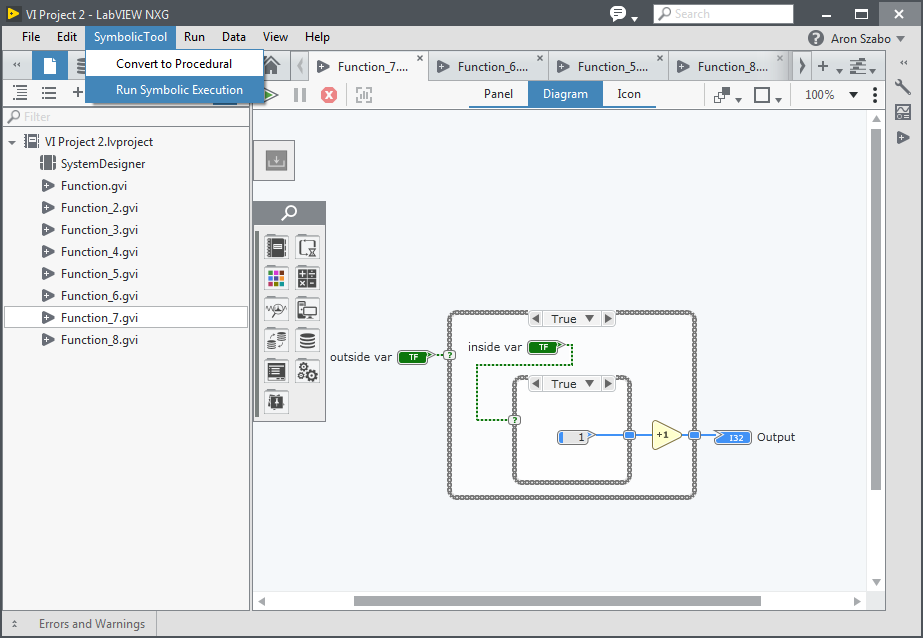
\includegraphics[width=150mm,keepaspectratio]{figures/interface.png}
\caption{Interface of LabVIEW NXG 2.1 with SymbolicTool installed} 
\label{fig:interface1}
\end{figure}

\paragraph{Debugging} Copy \verb|SymbolicTool.plugin.pdb| to the \verb|Addons| folder along with the DLL. Run LabVIEW and open a project. Select Debug / Attach to process... in Visual Studio and attach to \verb|LabVIEW NXG.exe|. Now the debugger in Visual Studio can be used.


%\label{page:last}
\end{document}
